
\section{Effectiveness as a platform \& navigations-per-add}

\subsection{Definitions}

A \textbf{navigation} is defined as

\onehalfspacing
\begin{itemize}
  \item a search, or
  \item a click on an instructor’s name, or
  \item a click on a crosslisted or prerequisite course link
\end{itemize}
\doublespacing

\noindent The \textbf{navigations-per-add} metric is the number of navigations taken by a user (within one session) before a section was added. 

To illustrate this metric, imagine that a user searches for ``{\tt csc}'' (one navigation so far) and begins to scroll through the list of courses. The user sees that Philip Guo is teaching CSC 210 and clicks on his name (two navigations so far), and then adds the section for CSC 210. \emph{A navigations-per-add of 2 is tallied for that user}. The user then clicks on the prerequisite for that class, CSC 172 (one navigation so far), and adds it. \emph{A navigations-per-add of 1 is tallied for that user}. The user then opens the list of labs embedded in 172 and adds one of them. \emph{A navigations-per-add of 0 is tallied for that user.} (Note that a value of 0 can also occur when a user scrolls through a list of courses and adds more than one of them without leaving the page.)

\subsection{General trends}

\begin{figure}
  \centering
  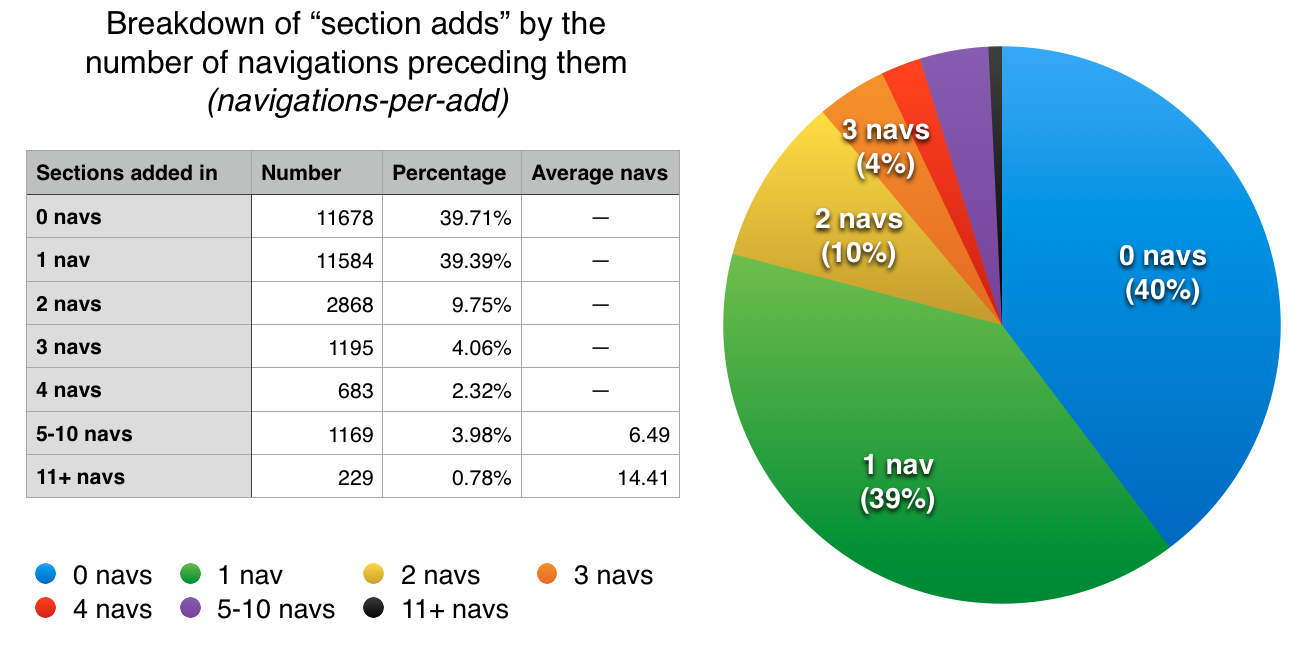
\includegraphics[width=1.0\textwidth]{images/graph/combined_navs}

  \caption{Frequency of different navigations-per-add values}
  \label{fig:navs-combined}
\end{figure}

Figure \ref{fig:navs-combined} shows the navigations-per-add breakdown for every time a section was added in Skedge. With 40\% of sections added in zero navigations and 39\% added within one navigation, it is immediately apparent that Skedge delivers users the content they look for in the vast majority of cases, assuming that the intention of the user was to add a course.

Considering the hypothesis claimed in Section 2.3.2 (that course selection criteria can be broken down to \emph{requirements}, \emph{electives}, and \emph{peer recommendations}), however, we ought examine if data for different use-cases are being conflated in this chart.

\subsection{Direct search (requirement criteria)}

  \begin{figure}
    \centering
    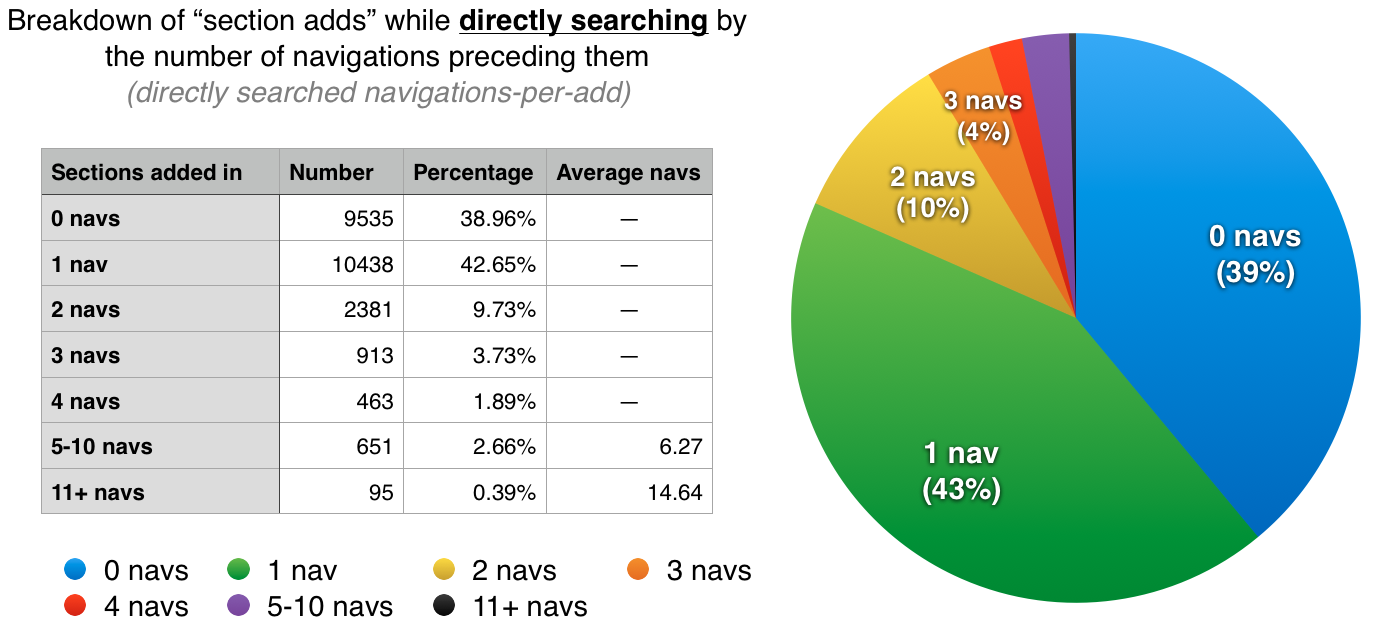
\includegraphics[width=1.0\textwidth]{images/graph/direct_navs}

    \caption{Frequency of navigations-per-adds for the goal of \emph{adding a specific course}}
    \label{fig:navs-direct}
  \end{figure}

  Direct searches are easy to distinguish, as we can take the subset of search queries that target a specific course, namely, those that \textbf{a)} contain both department and course code fields (e.g. ``{\tt csc 171}''), or \textbf{b)} contain a title field (``{\tt intro to programming}''). Figure \ref{fig:navs-direct} shows the navigations-per-add when, under this criteria, the user's goal was to add a specific course.

  The difference between these results and those in \ref{fig:navs-combined} is suble but logical. Users searching for a specific course should have an increased proportion of 1-navigation adds, as the graph shows, because the use-case is \emph{search for course}, \emph{add course}, perhaps occasionally taking an extra try to account for typos, not knowing the title or course code exactly, etc.

  But given this reasoning, why would 0-navigation adds still be so common in direct searches? Further analysis on only the sections that were added from direct search and with 0 navigations shows that 64\% of those sections are in fact \emph{subsections}. As happened in the illustrative example at the beginning of this section, this shows that a very common use-case is to add labs, workshops, etc. of a course directly after adding the main section.

  This hypothesis is further confirmed by doing the same analysis for ${navs}=1$ and ${navs}=2$, when the inverse behavior would be expected (it makes sense for subsections which were added seperately from their main sections to be more rate). Only 11\% of sections that were added from a direct search after 1 navigation are subsections, and that number drops to 8\% for 2 navigations.

\subsection{Browse (elective criteria)}

  \begin{figure}
    \centering
    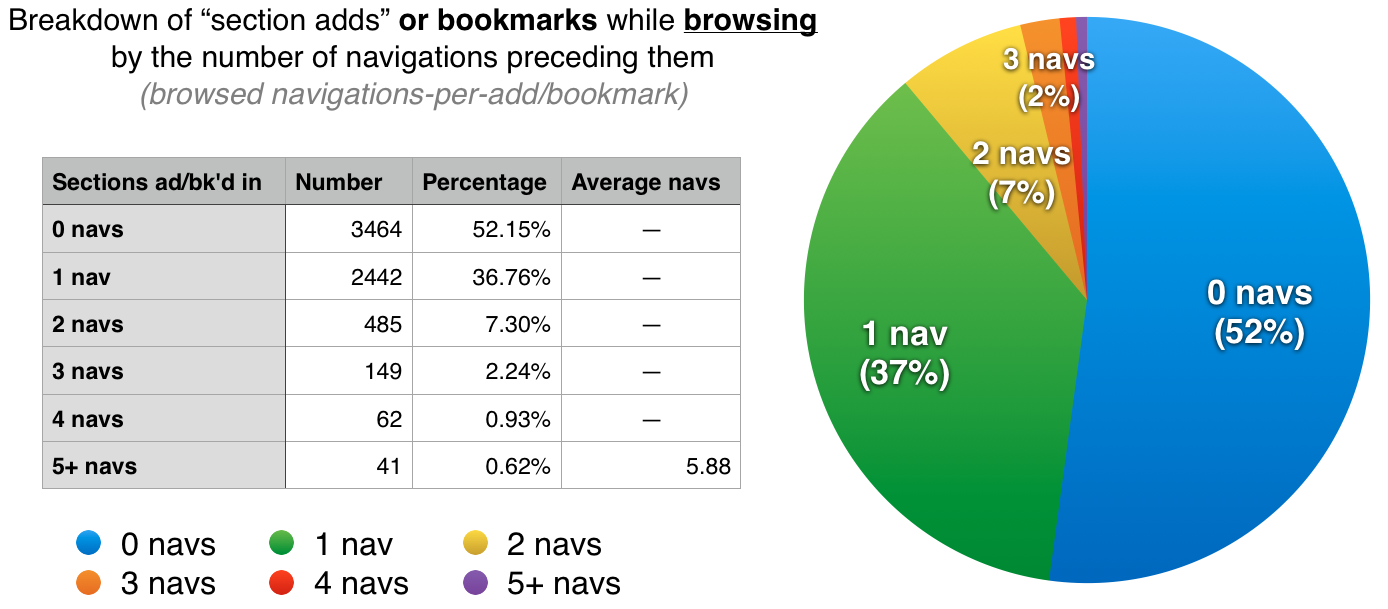
\includegraphics[width=1.0\textwidth]{images/graph/browsed_navs}

    \caption{Frequency of navigations-per-add/bookmark for the goal of \emph{browsing for courses}}
    \label{fig:navs-browse}
  \end{figure}

  Browsing behavior was done as a direct inverse of direct searches, detecting searches that didn't specifically target any courses. This time, bookmarks were also counted in a user's flow of events (i.e. they are treated the same as an add), because bookmarking is also a goal of course browsing behavior.

  The results are shown in Figure \ref{fig:navs-browse}. The difference between these results and the initial combined results of Figure \ref{fig:navs-combined} are more substantial than last time, and may defy expectations at first glance. While it may seem intuitive that browsed-for courses should have higher amounts of navigations, note that the graph itself is showing \emph{effectiveness} of such browsing. In this case, it makes sense that a significantly higher proportion of adds/bookmarks occur within zero navigations, because that indicates a high-level search and subsequent adds/bookmarks from that list instead of moving on to another search.

  As expected, and unlike the results of further direct-search analysis, the sections added/bookmarked when browsing within 0 navigations were mostly \emph{main} sections (only 37\% of them were subsections). This makes sense, as users may not be concerned with subsections if the goal of the browse is merely to mark interesting courses. This criterion saw more drastic drops in subsection amounts as well, as the number of navigations increased: 5\% subsections for ${navs}=1$, and 4\% subsections for ${navs}=2$.

\subsection{Peer-guided (recommendation criteria)}

  Given more time with Skedge Social being live and more forethought in tracking its usage, similar data analysis could be done on the subject of the effectiveness of Skedge in peer-guided course finding. Unfortunately, usage data to answer questions such as ``how many Facebook friends were listed as liking or taking a course when it was added?'' was not tracked, and cannot be retroactively computed due to Skedge's purposeful privacy limitations (Facebook friend data can only be retrieved client-side---no data is stored on the server that could authorize such a data request). Thus, part (c) of hypothesis \#2 cannot be verified.